\documentclass[tikz, border=8pt]{standalone}
\usepackage{tikz}
\usepackage{amsmath}
\usepackage{xcolor}

\usetikzlibrary{
  positioning,
  arrows.meta,
  fit,
  backgrounds,
  calc,
  decorations.pathreplacing
}

%% ── Colour palette ───────────────────────────────────────────────
\definecolor{clrInput}{HTML}{D6E4F7}
\definecolor{clrCNN}{HTML}{FDE8C8}
\definecolor{clrAttn}{HTML}{D8F5D8}
\definecolor{clrTrunk}{HTML}{EAD6F7}
\definecolor{clrFuse}{HTML}{FFF5CC}
\definecolor{clrActor}{HTML}{FAD4D4}
\definecolor{clrCritic}{HTML}{D4EEF7}
\definecolor{clrBorder}{HTML}{444444}
\definecolor{clrArrow}{HTML}{333333}

\tikzset{
  %% generic block
  blk/.style={
    draw=clrBorder, line width=0.6pt,
    rounded corners=2.5pt,
    font=\footnotesize,
    align=center,
    inner sep=4pt
  },
  %% typed blocks
  iblk/.style ={blk, fill=clrInput},
  cblk/.style ={blk, fill=clrCNN},
  ablk/.style ={blk, fill=clrAttn},
  fblk/.style ={blk, fill=clrFuse},
  tblk/.style ={blk, fill=clrTrunk},
  actblk/.style={blk, fill=clrActor},
  criblk/.style={blk, fill=clrCritic},
  outblk/.style={blk, fill=white, draw=clrBorder, dashed, line width=0.5pt},
  %% arrows
  arr/.style={-{Stealth[length=3.5pt, width=2.5pt]},
              line width=0.7pt, color=clrArrow},
  %% dim tags
  dim/.style={font=\scriptsize, color=gray!65}
}

\begin{document}
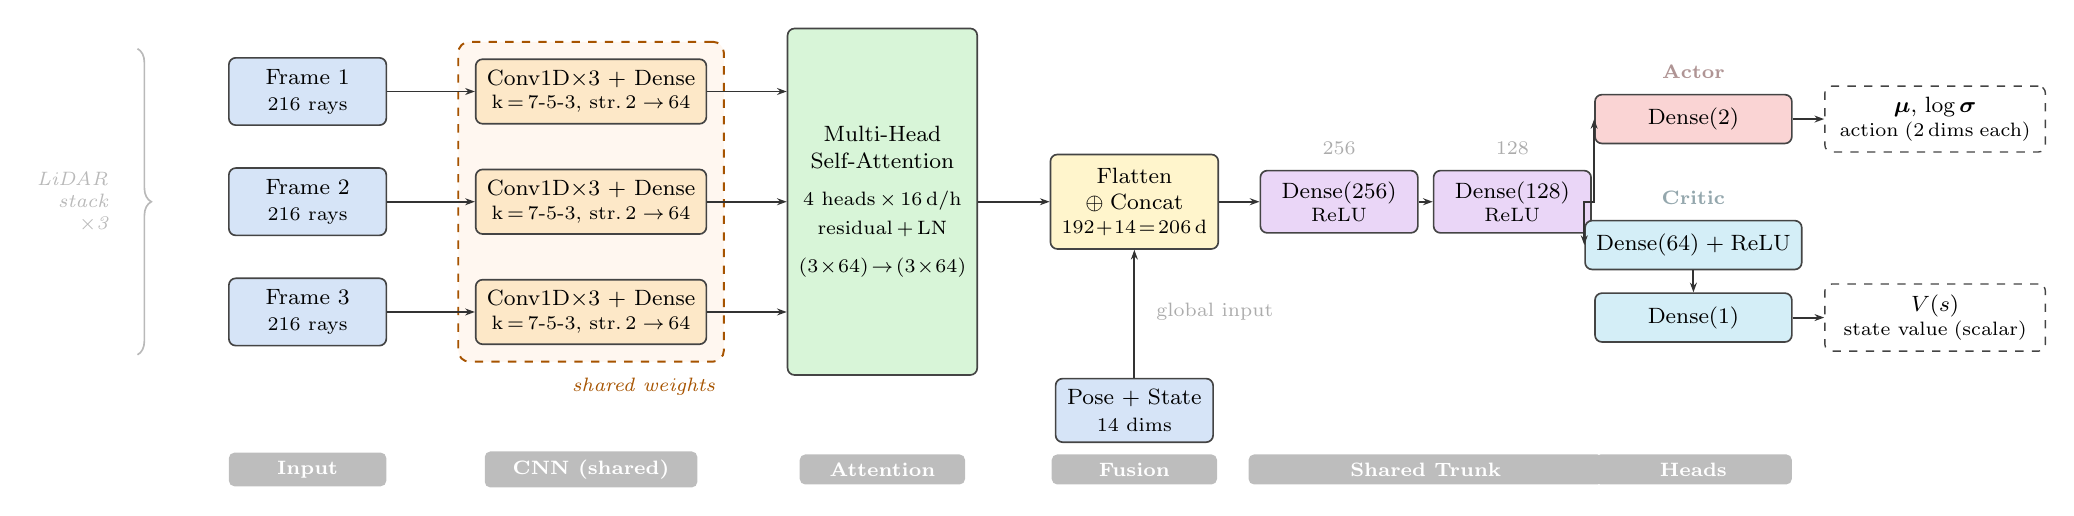
\begin{tikzpicture}

%% ================================================================
%%  X-POSITIONS  (centre of each stage, in cm)
%% ================================================================
%%  0.0 : input frames
%%  3.6 : CNN
%%  7.3 : attention
%% 10.5 : fusion / concat
%% 13.1 : Dense-256
%% 15.3 : Dense-128
%% 17.6 : actor head
%% 17.6 : critic head  (same x, different y)
%%
%%  Y-POSITIONS for the three parallel frame rows:
%%   +1.40 / 0.00 / -1.40  (before attention)
%%   0.00                   (after attention)

%% ================================================================
%%  STAGE 1 — Input
%% ================================================================
\node[iblk, minimum width=2.0cm, minimum height=0.70cm]
  (f1) at (0, 1.40) {Frame 1\\{\scriptsize 216 rays}};

\node[iblk, minimum width=2.0cm, minimum height=0.70cm]
  (f2) at (0, 0.00) {Frame 2\\{\scriptsize 216 rays}};

\node[iblk, minimum width=2.0cm, minimum height=0.70cm]
  (f3) at (0,-1.40) {Frame 3\\{\scriptsize 216 rays}};

%% left brace labelling the 3-frame LiDAR stack
\draw[decorate,
      decoration={brace, amplitude=5pt},
      line width=0.6pt, color=gray!55]
  ([xshift=-1.15cm, yshift= 3pt]f1.north west) --
  ([xshift=-1.15cm, yshift=-3pt]f3.south west)
  node[midway, left=7pt,
       font=\scriptsize\itshape, color=gray!55, align=right]
    {LiDAR\\stack\\$\times$3};

%% global state (will feed into fusion at x=10.5)
\node[iblk, minimum width=2.0cm, minimum height=0.70cm]
  (gs) at (10.5,-2.65) {Pose + State\\{\scriptsize 14 dims}};

%% ================================================================
%%  STAGE 2 — Shared-weight CNN
%% ================================================================
\node[cblk, minimum width=2.7cm, minimum height=0.72cm]
  (cnn1) at (3.6, 1.40)
  {Conv1D$\times$3 + Dense\\[-1pt]{\scriptsize k\,=\,7-5-3, str.\,2\;$\to$\,64}};

\node[cblk, minimum width=2.7cm, minimum height=0.72cm]
  (cnn2) at (3.6, 0.00)
  {Conv1D$\times$3 + Dense\\[-1pt]{\scriptsize k\,=\,7-5-3, str.\,2\;$\to$\,64}};

\node[cblk, minimum width=2.7cm, minimum height=0.72cm]
  (cnn3) at (3.6,-1.40)
  {Conv1D$\times$3 + Dense\\[-1pt]{\scriptsize k\,=\,7-5-3, str.\,2\;$\to$\,64}};

%% dashed box: shared weights
\begin{scope}[on background layer]
  \node[draw=orange!65!black, dashed, line width=0.7pt,
        fill=orange!6, rounded corners=4pt,
        fit=(cnn1)(cnn2)(cnn3), inner sep=6pt] (cnn_group) {};
\end{scope}
\node[font=\scriptsize\itshape, text=orange!65!black,
      below=2pt of cnn_group.south east, anchor=north east]
  {shared weights};

%% arrows  input → CNN
\draw[arr] (f1.east) -- (cnn1.west);
\draw[arr] (f2.east) -- (cnn2.west);
\draw[arr] (f3.east) -- (cnn3.west);

%% ================================================================
%%  STAGE 3 — Frame-stack attention
%% ================================================================
\node[ablk, minimum width=2.10cm, minimum height=4.40cm]
  (attn) at (7.3, 0)
  {Multi-Head\\Self-Attention\\[4pt]
   {\scriptsize 4 heads\,$\times$\,16\,d/h}\\[1pt]
   {\scriptsize residual\,+\,LN}\\[4pt]
   {\scriptsize $(3\!\times\!64)\!\to\!(3\!\times\!64)$}};

%% arrows  CNN → attention (horizontal entry at corresponding y)
\draw[arr] (cnn1.east) -- (cnn1.east -| attn.west);
\draw[arr] (cnn2.east) -- (attn.west);
\draw[arr] (cnn3.east) -- (cnn3.east -| attn.west);

%% ================================================================
%%  STAGE 4 — Fusion (flatten + concat)
%% ================================================================
\node[fblk, minimum width=2.10cm, minimum height=1.20cm]
  (concat) at (10.5, 0)
  {Flatten\\$\oplus$\;Concat\\[-1pt]{\scriptsize $192\!+\!14\!=\!206$\,d}};

%% arrows  attention → concat
\draw[arr] (attn.east) -- (concat.west);

%% global state → concat  (short vertical arrow)
\draw[arr] (gs.north) -- (concat.south);

%% label on the vertical arrow
\node[dim, right=3pt] at ($(gs.north)!0.52!(concat.south) + (0.05,0)$)
  {global input};

%% ================================================================
%%  STAGE 5 — Shared trunk
%% ================================================================
\node[tblk, minimum width=2.00cm, minimum height=0.65cm]
  (d256) at (13.1, 0) {Dense(256)\\[-1pt]{\scriptsize ReLU}};

\node[tblk, minimum width=2.00cm, minimum height=0.65cm]
  (d128) at (15.3, 0) {Dense(128)\\[-1pt]{\scriptsize ReLU}};

\draw[arr] (concat.east) -- (d256.west);
\draw[arr] (d256.east)   -- (d128.west);

\node[dim, above=2pt of d256] {256};
\node[dim, above=2pt of d128] {128};

%% ================================================================
%%  STAGE 6 — Actor / Critic heads
%% ================================================================

%% — Actor —
\node[actblk, minimum width=2.50cm, minimum height=0.62cm]
  (actor) at (17.6, 1.05)
  {Dense(2)};

\node[outblk, minimum width=2.80cm, minimum height=0.62cm,
      right=0.40cm of actor]
  (actor_out)
  {$\boldsymbol{\mu},\,\log\boldsymbol{\sigma}$\\[-1pt]
   {\scriptsize action\;(2\,dims\;each)}};

\draw[arr] (d128.east) -| (actor.west);
\draw[arr] (actor.east)  -- (actor_out.west);

%% actor label
\node[font=\scriptsize\bfseries, text=clrActor!70!black,
      above=2pt of actor] {Actor};

%% — Critic —
\node[criblk, minimum width=2.50cm, minimum height=0.62cm]
  (crit1) at (17.6,-0.55)
  {Dense(64)\;+\;ReLU};

\node[criblk, minimum width=2.50cm, minimum height=0.62cm,
      below=0.28cm of crit1]
  (crit2) {Dense(1)};

\node[outblk, minimum width=2.80cm, minimum height=0.62cm,
      right=0.40cm of crit2]
  (crit_out)
  {$V(s)$\\[-1pt]{\scriptsize state value\;(scalar)}};

\draw[arr] (d128.east) -| (crit1.west);
\draw[arr] (crit1.south) -- (crit2.north);
\draw[arr] (crit2.east)  -- (crit_out.west);

%% critic label
\node[font=\scriptsize\bfseries, text=clrCritic!70!black,
      above=2pt of crit1] {Critic};

%% ================================================================
%%  STAGE LABELS (bottom strip)
%% ================================================================
\def\labely{-3.40}

\begin{scope}[every node/.style={
    font=\scriptsize\bfseries, text=white,
    fill=gray!52, rounded corners=2pt,
    inner sep=3pt, align=center
  }]
  \node[minimum width=2.0cm]  at (0,    \labely) {Input};
  \node[minimum width=2.7cm]  at (3.6,  \labely) {CNN (shared)};
  \node[minimum width=2.1cm]  at (7.3,  \labely) {Attention};
  \node[minimum width=2.1cm]  at (10.5, \labely) {Fusion};
  \node[minimum width=4.50cm] at (14.2, \labely) {Shared Trunk};
  \node[minimum width=2.5cm]  at (17.6, \labely) {Heads};
\end{scope}

\end{tikzpicture}
\end{document}
